\documentclass[12pt]{article}
\usepackage[english]{babel}
\usepackage{natbib}
\usepackage{url}
\usepackage[utf8x]{inputenc}
\usepackage{amsmath}
\usepackage{graphicx}
\graphicspath{{images/}}
\usepackage{parskip}
\usepackage{fancyhdr}
\usepackage{vmargin}
\usepackage{xcolor}
\usepackage{siunitx}
\usepackage{physics}
\setmarginsrb{3 cm}{2 cm}{3 cm}{2 cm}{1 cm}{1.5 cm}{1 cm}{1.5 cm}

\title{Lab 02}													% Title
\author{G 03}														% Author
\date{26 Mar 2019}														% Date

\makeatletter
\let\thetitle\@title
\let\theauthor\@author
\let\thedate\@date
\makeatother

\pagestyle{fancy}
\fancyhf{}
\rhead{\theauthor}
\lhead{\thetitle}
\cfoot{\thepage}
\newcommand{\mis}[3]{(#1 \pm #2) \ #3}
\newcommand{\misp}[3]{(#1 \#3 \pm #2}
\begin{document}

%%%%%%%%%%%%%%%%%%%%%%%%%%%%%%%%%%%%%%%%%%%%%%%%%%%%%%%%%%%%%%%%%%%%%%%%%%%%%%%%%%%%%%%%%

\begin{titlepage}
	\centering
    \vspace*{0.5 cm}
    
\includegraphics[scale = 0.75]{polito.jpg}\\[1.0 cm]				% University Logo
    \textsc{\LARGE Politecnico di Torino}\\[2.0 cm]						% University Name
	\textsc{\Large Digital systems electronics\\ A.A. 2018/2019}\\[0.5 cm]		% Course Code
	\textsc{\Large Prof. G. Masera}\\[0.5 cm]		% Nome del Professore
	\rule{\linewidth}{0.2 mm} \\[0.4 cm]
	{ \huge \bfseries \thetitle \\ \small \thedate}\\
	\rule{\linewidth}{0.2 mm} \\[1.5 cm]
	
	\begin{minipage}{0.4\textwidth}
		\begin{flushleft} \large
			Berchialla Luca\\												%Cognomi e nomi
			Laurasi Gjergji
			\\
			
			Mattei Andrea\\
            Lombardo Domenico Maria\\
            
			\end{flushleft}
			\end{minipage}~
			\begin{minipage}{0.4\textwidth}
            
			\begin{flushright} \large
			236032\\													%Matricole
			238259\\
            233755\\
            233959\\
            
		\end{flushright}
        
	\end{minipage}\\[2 cm]
	
\end{titlepage}

%%%%%%%%%%%%%%%%%%%%%%%%%%%%%%%%%%%%%%%%%%%%%%%%%%%%%%%%%%%%%%%%%%%%%%%%%%%%%%%%%%%%%%%%%

\section{ Controlling a 7-segments display}

	Figure 1 shows a 7-segment decoder module whose input bits $C2 C1 C0$ drive a 7 segment display through the bits $HEX0_{0}->HEX0_{6}$ 
	
	\begin{figure}[h]
		\centering
		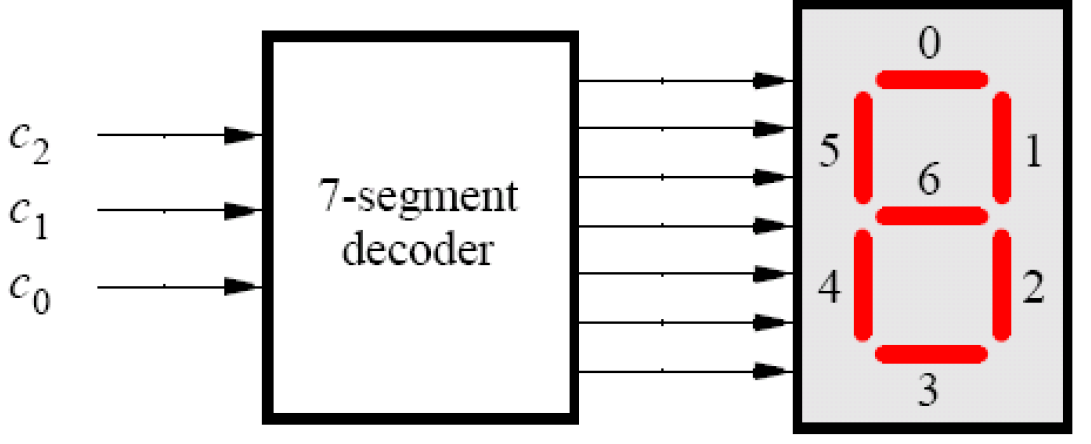
\includegraphics[scale = 0.7]{Niki_puntoA/system.png}
		\caption{7-segment decoder + display}
	\end{figure}	

	Figure 2 shows the truth table to be implemented for the 7-segment decoder. As shown just the characters $H E L O$ will be implemented.
	The sequent logical states can be easily derived from the table:
	\[HEX6=\overline{C2}\cdot\overline{C1}\]
	\[HEX5=\overline{C2}\]
	\[HEX4=\overline{C2}\]
	\[HEX3=\overline{C2}\cdot(C0+C1)\]
	\[HEX2=\overline{C2}\cdot\overline{C1}\cdot\overline{C0}+\cdot\overline{C2}\cdot C1\cdot C0\]
	\[HEX1=\overline{C2}\cdot\overline{C1}\cdot\overline{C0}+\cdot\overline{C2}\cdot C1\cdot C0\]
	\[HEX0=\overline{C2}\cdot C0\]
	

	\begin{figure}[h]
		\centering
	 	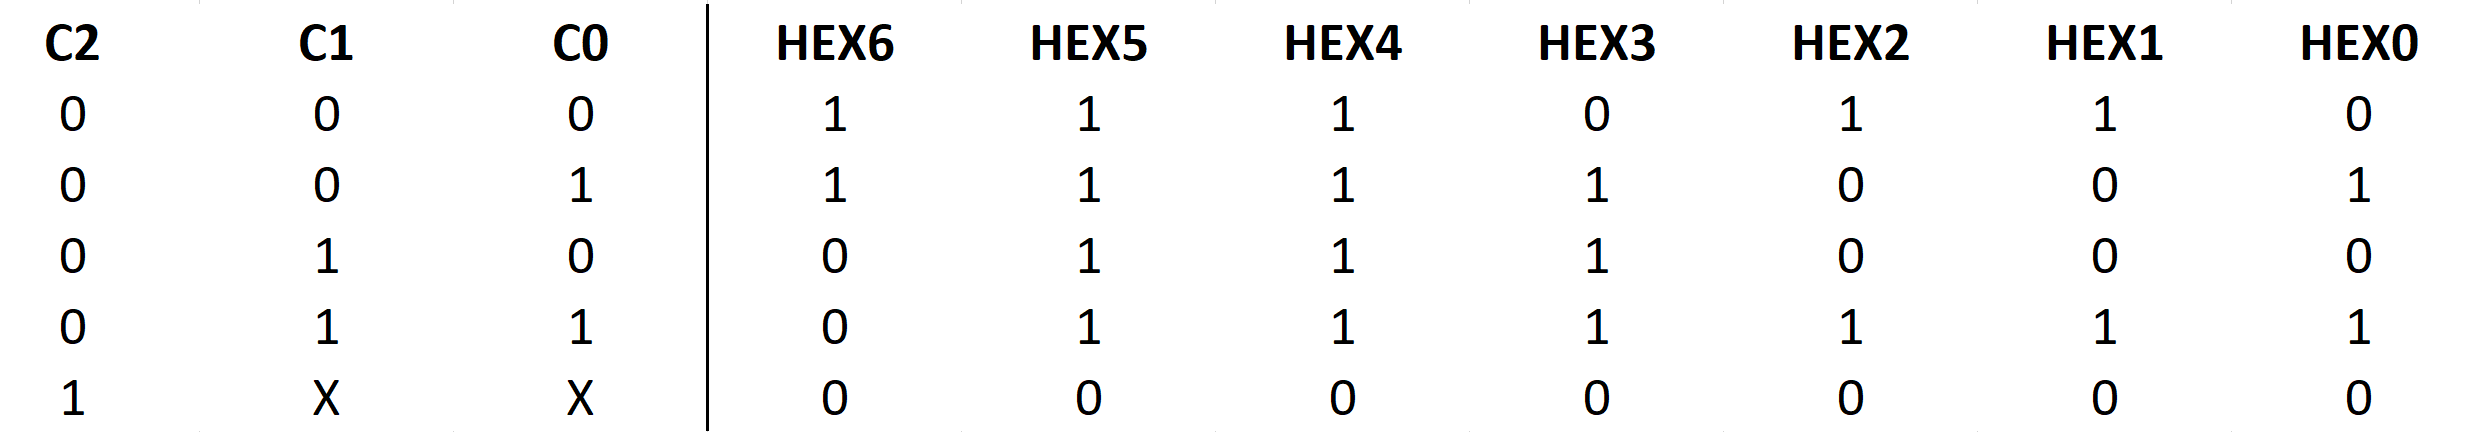
\includegraphics[scale = 0.45]{Niki_puntoA/tabella.png}
	 	\caption{decoder truth table}
	\end{figure}	
	 
	 Finally the logic states are implemented using gates as shown in $figure 3$.\newline
	 The circuit is then described into VHDL using a dataflow style approach, the VHDL file is called $puntoA.vhd$. 
	 
	 
	 
	  \begin{figure}[!h]
	  \centering
	  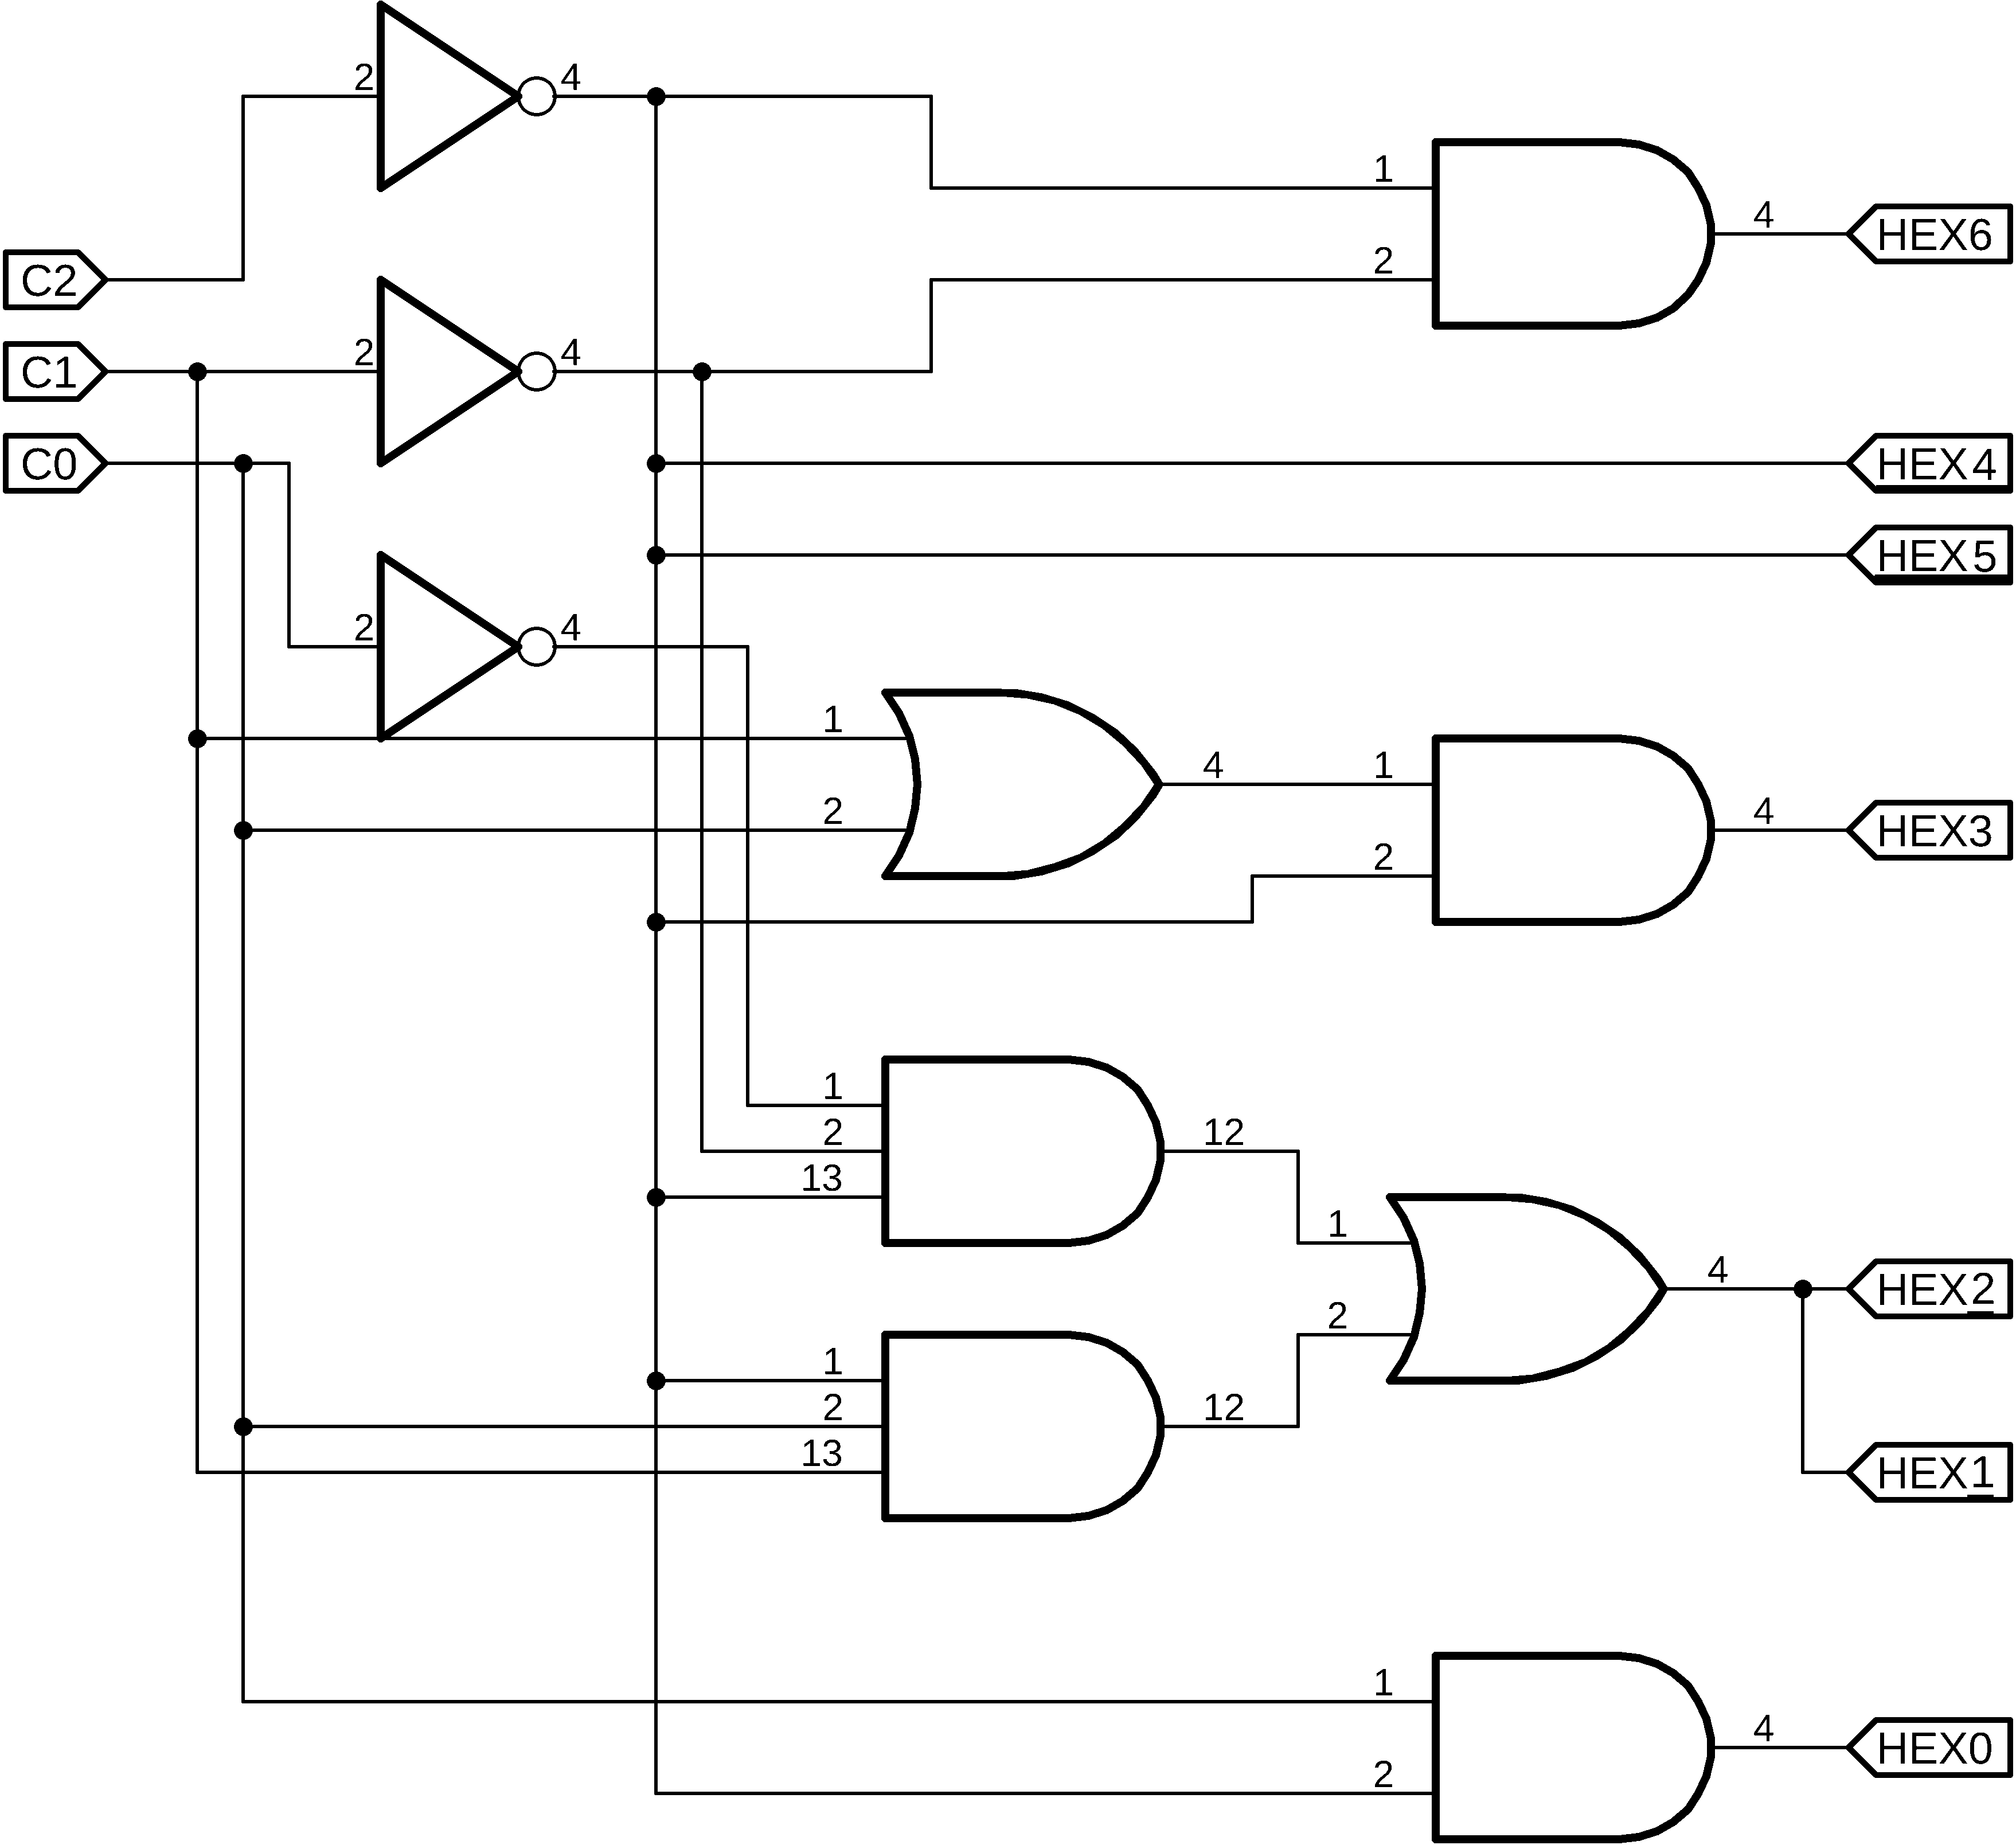
\includegraphics[scale = 0.65]{Niki_puntoA/schema.png}
	  \caption{decoder gates implementation}
  	\end{figure}		
  
  The VHDL entry has been finally simulated via  $testbench approach$ where every possible input combination has been considered validating the output.
  The testbench results are shown below in figure 4.
  
  \begin{figure}[!h]
  	\centering
  	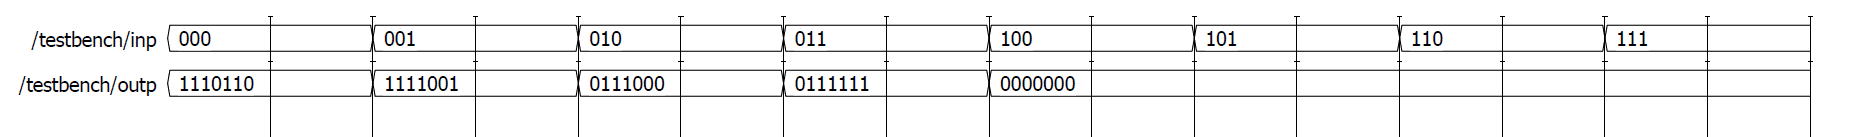
\includegraphics[scale = 0.65]{Niki_puntoA/Capturef.png}
  	\caption{Testbench results}
  \end{figure}





\section{ Multiplexing the 7-segments display output}
\begin{figure}[h]
	\centering
	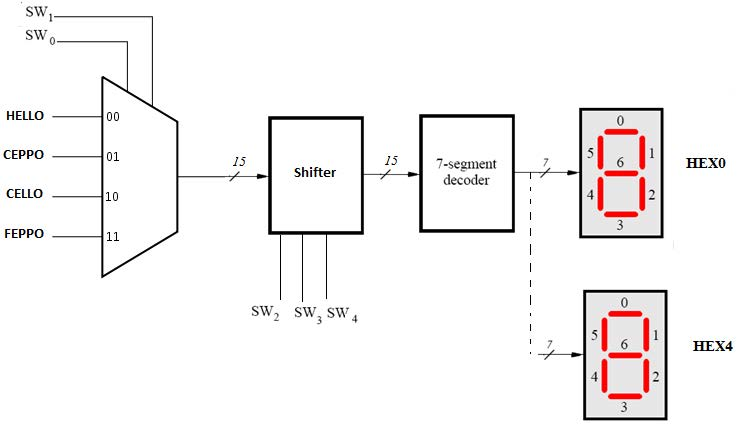
\includegraphics[scale = 0.7]{Berchialla_PuntoB/image1.jpg}
	\caption{multiplexer + shifter + 7-segment decoder + display}
\end{figure}
	Figure 5 shows the architecture of the implemented circuit. It is composed by a three-bit wide 4-to-1 multiplexer, which has the data inputs fixed to the words we want to display following the codification of figure 6. A shifter that rotates the selected word in a circular fashion and 5 7-segments decoders followed by their respective displays.


\begin{figure}[h]
	\centering
	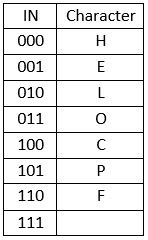
\includegraphics[scale = 0.4]{Berchialla_PuntoB/image2.jpg}
	\caption{7-segment display character codes}
\end{figure}

Each sub-circuit has been implemented and tested separately than in the $Part2$ entity all components are used to describe the circuit.

\subsection{Multiplexer}
Each letter code has been assigned to a signal for code readability. Than the output of the multiplexer has been described using the $when$ structure.\newline
The testbench of this component assigns all possible combinations of the selection inputs, then the output is checked using the waveforms.
\subsection{Shifter}
The shifter output has been set as a concatenation of two parts of the input for meaningful input and forced to zero for all other inputs. The behaviour implemented is described in $figure 7$.
\begin{figure}[h]
	\centering
	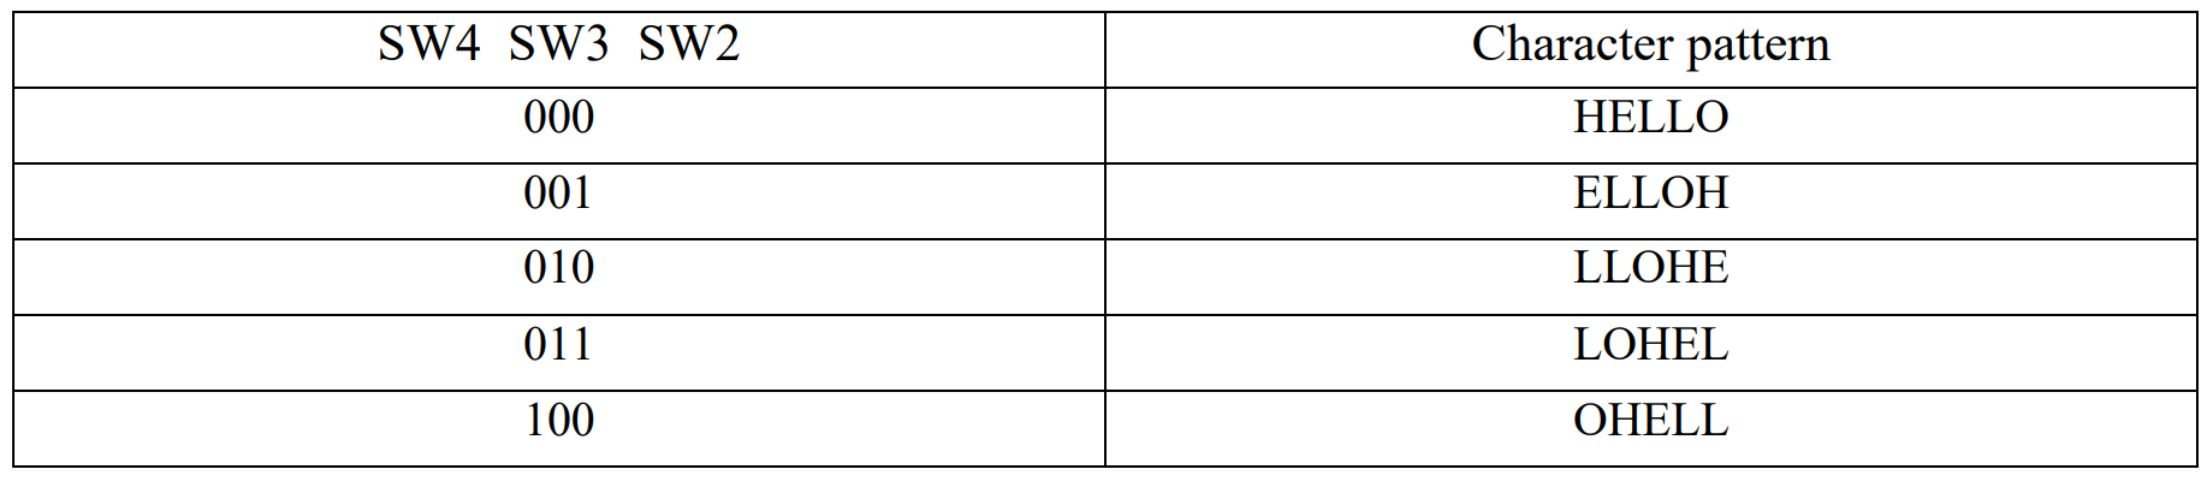
\includegraphics[scale = 0.2]{Berchialla_PuntoB/image3.jpg}
	\caption{Example of shifter behaviour with the word "HELLO"}
\end{figure}
This component has been tested by fixing the input to a concatenation of 5 3-bit binary numbers in rising order and assigning all possible combination of the $SW$ inputs. Than the behaviour has been checked in the simulated waveforms.
\subsection{7-segment decoder}
This component could have been reused from the previous point but it has been quickly reimplemented behaviourally to be able to display also the letters $C$,$P$, and $F$. Although, the testbench was reused taking care to verify also the new letters in the waveform simulation.
\subsection{Testbench of the whole circuit}
To be able to verify the correct behaviour of the circuit several signals have been created. \newline
A signal for each letter with values for each letter corresponding to the 7 bits of the display code.
An $error$ signal that is used as a flag to quickly detect possible errors.\newline
In the port map the displays are assigned in inverse order to test view the output in the simulation with the first letter in the $HEX0$ display instead of the $HEX4$ display.\newline
The circuit first tested by fixing the multiplexer selection to $00$ corresponding to the $HELLO$ word and assigning all the possible combinations to the shifter selection inputs. With several if statements the cycling of the $HELLO$ word is checked. \newline
Than the shifter selection inputs are forced to $000$ and is verified that all the other words are displayed properly.
\section{ Binary to Decimal converter}
punto 3
\section{ Binary-to-BCD Converter}
punto 4



\end{document}
